% --------------------------------------------------------------
% This is all preamble stuff that you don't have to worry about.
% Head down to where it says "Start here"
% --------------------------------------------------------------

\documentclass[12pt]{article}

\usepackage[margin=1in]{geometry} 
\usepackage{amsmath,amsthm,amssymb}
\usepackage{color}
\usepackage{tikz, pgfplots}
\usepackage{graphicx}
\usepackage{epstopdf} %converting to PDF
\usepackage{subcaption}

\makeatletter

\renewcommand\section{\@startsection {section}{1}{\z@}%
	{-3.5ex \@plus -1ex \@minus -.2ex}%
	{2.3ex \@plus.2ex}%
	{\normalfont\large\bfseries}}% from \Large
\renewcommand\subsection{\@startsection{subsection}{2}{\z@}%
	{-3.25ex\@plus -1ex \@minus -.2ex}%
	{1.5ex \@plus .2ex}%
	{\normalfont\large\bfseries}}% from \large
\makeatother

\begin{document}
	
	% --------------------------------------------------------------
	%                         Start here
	% --------------------------------------------------------------
	
	%\renewcommand{\qedsymbol}{\filledbox}
	
	\title{\textbf{Pattern Recognition Assignment \#{1}}\\
	Universit{\'e} de Fribourg}%replace X with the appropriate number
	\author{{Lin Bai, 09935404}} %replace with your name
	
	\maketitle
	
	%%%%%%%%%%%%%%%%%%%%%%%%%%%%%%%%%%%%%%%%%%%%%%%%%%%%%%%%%%%%%%%%%%%%%%%%%%%%%%%%%%%%%%%%
	%%%%%%   notations
	%%%%%%%%%%%%%%%%%%%%%%%%%%%%%%%%%%%%%%%%%%%%%%%%%%%%%%%%%%%%%%%%%%%%%%%%%%%%%%%%%%%%%%%%
	\section{Source Code}
	Attached to this report.

	%%%%%%%%%%%%%%%%%%%%%%%%%%%%%%%%%%%%%%%%%%%%%%%%%%%%%%%%%%%%%%%%%%%%%%%%%%%%%%%%%%%%%%%%
	%%%%%%   question 1, sub question (a)
	%%%%%%%%%%%%%%%%%%%%%%%%%%%%%%%%%%%%%%%%%%%%%%%%%%%%%%%%%%%%%%%%%%%%%%%%%%%%%%%%%%%%%%%%
	\section{Analysis}
	This k-NN algorithm is implemented using two kinds of distance, $Euclidean$ and $Manhattan$. The $k$ values are 1, 3, 5, 10, 15.\\
	\\
	Their accuracy are listed in the table bellow.\\
	\begin{table}[htbp]
		\centering
		\label{my-label}
		\begin{tabular}{l|l|l|l|l|l}
			\hline
			          & k = 1 & k = 3 & k = 5 & k = 10 & k = 15 \\
			\hline
			Euclidean &       &       &       &       & \\
			\hline
			Manhattan &       &       &       &       &  \\
			\hline
		\end{tabular}
	\end{table}



	\begin{figure}[!h]
	\centering
		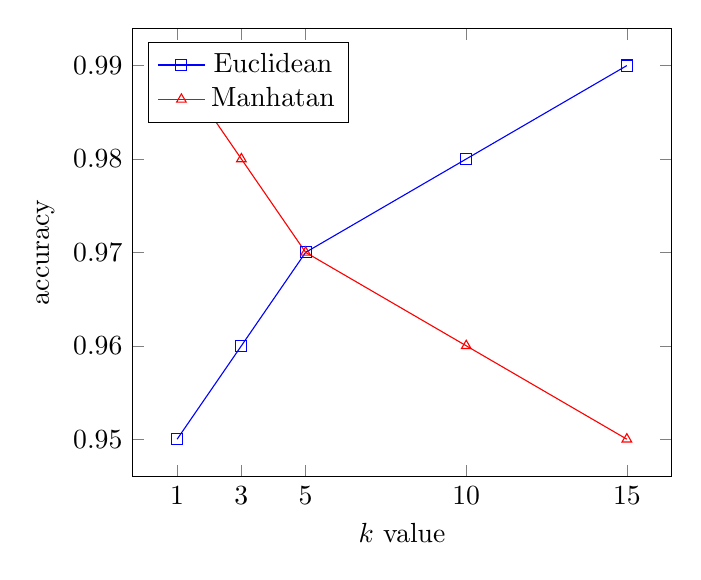
\begin{tikzpicture}
			\centering
			\begin{axis}[
			xtick={1,3,5,10,15},
			ytick={0.95,0.96,0.97,0.98,0.99,1.00},
			legend pos=north west,
			xlabel = $k$ value,
			ylabel = accuracy,
			]
			
			\addplot[
			color=blue,
			mark=square,
			]
			coordinates {
				(1,0.95)(3,0.96)(5,0.97)(10,0.98)(15,0.99)
			};
			\addlegendentry{Euclidean}
			
			\addplot[
			color=red,
			mark=triangle,
			]
			coordinates {
				(1,0.99)(3,0.98)(5,0.97)(10,0.96)(15,0.95)
			};
			\addlegendentry{Manhatan}
			
			
			\end{axis}
		\end{tikzpicture}
	\end{figure}

	
	% --------------------------------------------------------------
	%     You don't have to mess with anything below this line.
	% --------------------------------------------------------------
	
\end{document}